\chapter{Bluetooth}
\label{Bluetooth}
% ================ Einstellungen =======================
\thispagestyle{fancy} \rhead{\slshape Bluetooth}
% ======================================================
In diesem Kapitel wird der gesamte Bluetooth-Teil, also alle Komponenten und Konfigurationen, die zum Empfangen und verwerten der Daten benötigt werden, genauer erläutert. Es folgt daher zuerst eine Aufteilung nach Hardwarekomponenten und danach Softwareteil. 

\section{Beacons im Museum}
Beacons sind kleine und kompakte Bluetooth-Sender die auf der Low Energy Spezifikation basieren. Sie können entweder batteriebetrieben oder mit permanentem Stromanschluss an Räumen oder Objekten installiert werden\cite{TechTag}. Bewegt sich ein Museumsbesucher in die Nähe eines Beacons mit diesem Dojo, so kann er Audio- und Video-Beiträge empfangen und mit dem Dojo abspielen. Zudem kann an der Kasse des Museums entschieden werden, welche Zonen aktiviert werden sollen. Das Dojo beinhaltet somit auch die Zutrittsberechtigungen. Der Vorteil dieses Systems ist der Preis. Es wird nur so viel bezahlt, was den Kunden  interessiert.	

\section{Minew E7}
Mit dem Beacon Minew E7 konnte ein Museum simuliert werden, um den Prototypen auf die Funktionalität zu prüfen. Dieser Beacon lässt sich über die gratis App BeaconSET+  konfigurieren. Dieser Beacon bringt einige Vorteile mit sich. Zum einen kriegt er eine maximale Reichweite von 100 m  hin, doch noch viel wichtiger ist das Protokoll. Der Minew E7 unterstützt iBeacon und Eddystone Protokolle die entweder separat oder gleichzeitig benutzt werden können. \cite{beaconshop24}

\section{Bluetooth-Modul HM-11}
Das HM-11 Bluetooth-Modul benötigt eine Versorgungsspannung von 3.3 V DC und verfügt über das Kommunikationsprotokoll UART. Die Standard Baudrate beträgt 9600bps und nimmt beim Senden einen Strom von 15 mA auf. In offener Umgebung beträgt die Reichweite bis zu 30 m und unterstützt AT Kommandos, um das Bluetooth-Modul zu konfigurieren. Mit diesem Modul werden die Daten, die von einem Beacon ausgesendet werden, empfangen.  

\section{Bluetooth-Konfiguration}
Damit der Prototyp die Beacons erkennt, wird das bereits oben erwähnte HM-11 Modul, verwendet. Es ermöglicht das Empfangen der Identifikationsnummer von dem Beacon. Um eine reibungslose Kommunikation zu gewährleisten, müssen einige Konfigurationen beim Bluetooth-Modul vorgenommen werden. Das Modul wird mit einem FTDI verkabelt und am PC angeschlossen. Mit den AT-Kommandos wie AT+Name, AT+ROLE1, AT+IMME1 und AT+DISI? kann das Bluetooth-Modul nun eingestellt werden. Falls das Bluetooth-Modul bereits auf dem Print bestückt ist, kann es über die UART-Schnittstelle konfiguriert werden. 

\section{Protokollbeschreibung}
Das iBeacon-Protokoll wurde von Apple entwickelt und baut auf der Bluetooth-Low-Energy-Spezifikation auf. Das Paket das ausgestrahlt wird hat eine Länge von 30 Byte. In diesem Paket stecken die ganzen Informationen wie Geräte-ID, Beacon-Typ, Referenzempfangsleistung und noch viele weitere Daten drin. Um die Beacons zu scannen, wurde die Software so geschrieben, dass es nur die UUID, den Majorvalue und den RSSI-Wert benötogt. Nachfolgend wird der RSSI-Wert genauer beschrieben sowie der Aufbau des iBeacons-Paket graphisch dargestellt. \cite{Indoorpos}

%%%%%%
\begin{figure}[htp]
\centering
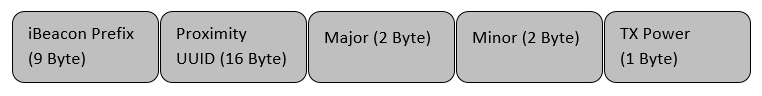
\includegraphics[width=15cm]{Bilder/iBeacon_Paket.PNG}
\caption{Aufbau eines iBeacon-Pakets}
\label{fig:iBeacon}
\end{figure}
%%%%%%

\section{Receiver Signal Strength Indicator (RSSI)}
Der RSSI ist ein dimensionsloser Wert. Er beschreibt die empfangene Leistung bei kabelloser Kommunikation. Angegeben wird der Wert in dBm, was das Verhältnis in Dezibel zwischen der Leistung mW und der Referenzleistung 1 mW darstellt.
\begin{equation}
    RSSI = -(10n\,log_{10}\,d+a)
\end{equation}
Dabei gilt: \\
\hspace*{10mm}
n = umgebungsabhängiger Dämpfungswert \\
\hspace*{10mm}
d = Distanz zwischen dem Sender und dem Empfänger \\
\hspace*{10mm}
a = empfangene Signalstärke des Senders in einem Abstand von einem Meter \\
\newpage
\section{IBeacons auslesen und identifizieren}
Mittels der Funktion scan() im State SCAN wird mit dem hm-11 nach den verfügbaren IBeacons in der Umgebung gesucht. Über eine serielle Schnittstelle (UART) wird vom MCU der Befehl AT+DISI? dem hm-11 geschickt, wobei als Antwort dann alle umliegenden IBeacons in einem String zurückkommen (siehe Abbildung \ref{fig:disiCommand}).\\
\begin{figure}[h]
\centering
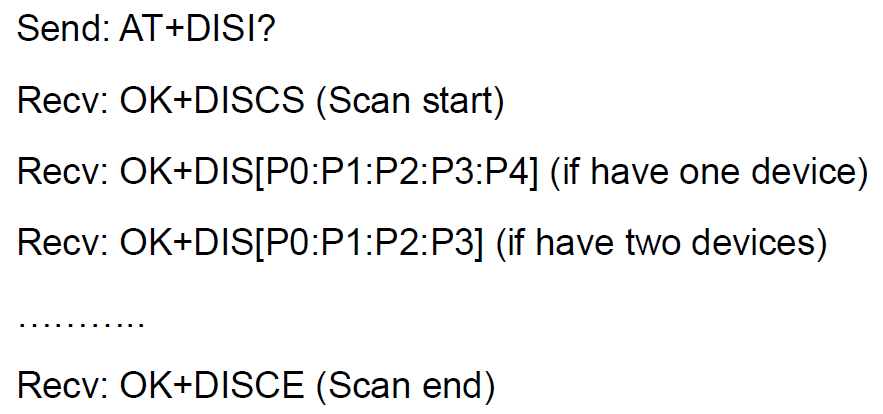
\includegraphics[scale=0.7]{Bilder/disi_command.PNG} 
\caption[Rückgabe des AT+DISI? Befehls]{P0: Factory ID (8 Byte); P1: IBeacon UUID (32 Byte); P2: Major-, Minorvalue, Measured Power (10 Byte); P3: Media-Access-Control-Adresse MAC (12 Byte); P4: RSSI (4 Byte) \cite{hm11Datasheet}}
\label{fig:disiCommand}
\end{figure}
Dafür wird vom MCU jeder char, rsp. jedes Byte vom Datenbuffer ausgelesen und verwertet. Es wird zuerst nach einer UUID eines IBeacons gefiltert und dann die ersten drei Zahlen in einen Integer gecastet. Anschließend soll das Majorvalue\footnote{Major- und Minorvalues dienen hauptsächlich zur zusätzlichen Identifikation eines IBeacons}, welches einen bestimmten, selbst wählbaren Wert hat, abgeglichen werden, damit nur die IBeacons berücksichtig werden, die relevant sind. Ist der empfangene RSSI-Wert grösser als -90dbm, wird der IBeacon eingespeichert. Dies wird mit jedem empfangenen IBeacon wiederholt und immer die RSSI-Werte miteinander verglichen, wobei dann der IBeacon mit dem grösseren RSSI-Wert ins System gespeichert und als Returnvalue von der scan() Funktion zurückgegeben wird.

\section{Validierung}
Für die Validierung wurden zwei IBeacons mit Androidhandys simuliert (Beacon Simulator App). Dafür wurden diese mit einer Distanz von ungefähr $6m$ zueinander auf einer Höhe von ca. $2m$ platziert. Um die detektierten IBeacons direkt auszuwerten, wurde die UUID auf einen Emulator (Putty) über eine serielle Schnittstelle (USB Typ micro B) herausgeschrieben. Somit konnte verifiziert werden, dass der vom Dojo detektierte IBeacon auch der sich am Dojo nächsten befindliche IBeacon war. 
\\[0.5cm]
Eine definitive Distanzbestimmung zwischen dem IBeacon und dem Dojo ist schwierig, da die Sendeleistung der simulierten IBeacons etwas schwanken. Auch die Auslegung des Raumes, sowie die Einrichtung kann das Signal abschwächen, was direkten Einfluss auf die Erkennungsdistanz hat. Es kann aber festgehalten werden, dass ein IBeacon in einem Umkreis von $3m$ garantiert erkennt wird, solange sich keine Gegenstände unmittelbar zwischen den beiden Objekten befinden.